\documentclass[12pt,a4paper]{article}

% ─── Encoding & fonts ───
\usepackage[utf8]{inputenc}
\usepackage[T1]{fontenc}

% ─── Page layout ───
\usepackage[margin=2.5cm]{geometry}

% ─── Math ───
\usepackage{amsmath,amssymb,amsthm,mathtools}

% ─── Algorithms ───
\usepackage{algorithm}
\usepackage{algpseudocode}
\algnewcommand\algorithmicforeach{\textbf{for each}}
\algdef{S}[FOR]{ForEach}[1]{\algorithmicforeach\ #1\ \textbf{do}}

% ─── TikZ ───
\usepackage{tikz}
\usetikzlibrary{shapes.geometric,arrows.meta,positioning,fit,
                backgrounds,calc,decorations.pathreplacing,matrix,chains}

% ─── Tables ───
\usepackage{booktabs}
\usepackage{tabularx}
\usepackage{multirow}
\usepackage{array}
\usepackage{float}

% ─── Code listings ───
\usepackage{listings}
\usepackage{xcolor}

% ─── Misc ───
\usepackage{caption}
\usepackage{subcaption}
\usepackage{enumitem}
\usepackage{hyperref}
\hypersetup{colorlinks=true,linkcolor=blue!70!black,
            pdftitle={retriever.py Annotated Reference}}

% ─── Headers / footers ───
\usepackage{fancyhdr}
\pagestyle{fancy}
\fancyhf{}
\lhead{\footnotesize MIVA-KNIGHT \texttt{retriever.py} --- Annotated Technical Reference}
\rhead{\footnotesize IT 581 Project}
\cfoot{\thepage}

% ─── Theorem environments ───
\theoremstyle{definition}
\newtheorem{theorem}{Theorem}[section]
\newtheorem{lemma}[theorem]{Lemma}
\newtheorem{definition}[theorem]{Definition}
\newtheorem{axiom}[theorem]{Axiom}
\newtheorem{proposition}[theorem]{Proposition}
\newtheorem{corollary}[theorem]{Corollary}
\newtheorem{invariant}[theorem]{Invariant}
\theoremstyle{remark}
\newtheorem{remark}[theorem]{Remark}

% ─── Colours ───
\definecolor{cBlue}{RGB}{220,230,245}
\definecolor{cGreen}{RGB}{210,240,210}
\definecolor{cOrange}{RGB}{255,235,215}
\definecolor{cGray}{RGB}{230,230,230}
\definecolor{cPurple}{RGB}{235,220,245}
\definecolor{cTeal}{RGB}{200,235,235}
\definecolor{cYellow}{RGB}{255,248,200}
\definecolor{cDark}{RGB}{40,60,100}
\definecolor{cRed}{RGB}{245,220,220}
\definecolor{cMed}{RGB}{200,240,230}
\definecolor{cKG}{RGB}{245,235,200}
\definecolor{cFAISS}{RGB}{210,225,255}

% ─── Code style ───
\lstset{
  language=Python,
  basicstyle=\ttfamily\footnotesize,
  keywordstyle=\color{blue!70!black}\bfseries,
  commentstyle=\color{green!50!black}\itshape,
  stringstyle=\color{orange!70!black},
  numberstyle=\tiny\color{gray},
  frame=single, rulecolor=\color{gray!40},
  numbers=left, breaklines=true,
  tabsize=4, showstringspaces=false,
  morekeywords={dataclass,abstractmethod,ABC,Optional,List,
                RetrievedDocument,RetrieverOutput}
}

% ─── TikZ styles ───
\tikzset{
  basebox/.style={rectangle,rounded corners=4pt,draw=black!60,
                  align=center,font=\footnotesize},
  bluenode/.style={basebox,fill=cBlue,minimum width=3cm,
                   minimum height=0.85cm},
  greennode/.style={basebox,fill=cGreen,minimum width=3cm,
                    minimum height=0.85cm,thick},
  orangenode/.style={basebox,fill=cOrange,minimum width=3cm,
                     minimum height=0.85cm},
  graynode/.style={basebox,fill=cGray,minimum width=3cm,
                   minimum height=0.85cm},
  purplenode/.style={basebox,fill=cPurple,minimum width=3cm,
                     minimum height=0.85cm},
  tealnode/.style={basebox,fill=cTeal,minimum width=3cm,
                   minimum height=0.85cm},
  kgnode/.style={basebox,fill=cKG,minimum width=3cm,
                 minimum height=0.85cm,draw=orange!60},
  faissnode/.style={basebox,fill=cFAISS,minimum width=3cm,
                    minimum height=0.85cm,draw=blue!50,thick},
  mednode/.style={basebox,fill=cMed,minimum width=3cm,
                  minimum height=0.85cm,thick},
  warnnode/.style={basebox,fill=cRed,minimum width=3cm,
                   minimum height=0.85cm},
  decnode/.style={diamond,draw=black!70,fill=cYellow,aspect=2.8,
                  align=center,font=\scriptsize},
  arr/.style={->,>=Stealth,thick,color=black!70},
  thkarr/.style={->,>=Stealth,very thick,color=cDark},
  dasharr/.style={->,>=Stealth,dashed,thick,color=gray!60},
  redarr/.style={->,>=Stealth,thick,color=red!60!black},
  grnarr/.style={->,>=Stealth,thick,color=green!50!black},
  bluarr/.style={->,>=Stealth,thick,color=blue!60!black},
  ornarr/.style={->,>=Stealth,thick,color=orange!70!black}
}

\renewcommand{\algorithmicrequire}{\textbf{Input:}}
\renewcommand{\algorithmicensure}{\textbf{Output:}}

%───────────────────────────────────────────────────
\begin{document}

% ══════════════════════════════════════════════════
%  TITLE PAGE
% ══════════════════════════════════════════════════
\begin{titlepage}
\centering\vspace*{1.5cm}
{\Huge\bfseries\color{cDark} MIVA-KNIGHT}\\[0.4cm]
{\Large\bfseries \texttt{retriever.py}}\\[0.3cm]
{\large Annotated Mathematical \& Algorithmic Reference}\\[1.0cm]

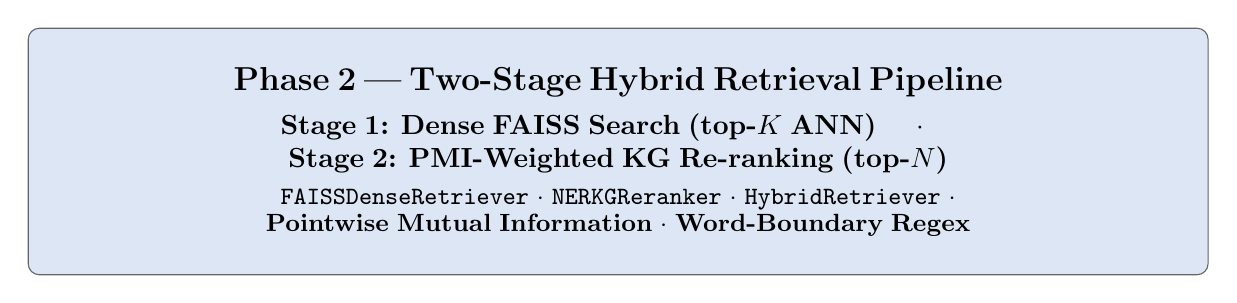
\begin{tikzpicture}
  \node[basebox,fill=cBlue,text width=14cm,inner sep=14pt]{
    \large\bfseries Phase 2 --- Two-Stage Hybrid Retrieval Pipeline\\[4pt]
    \normalsize
    Stage 1: Dense FAISS Search (top-$K$ ANN) $\quad\cdot\quad$
    Stage 2: PMI-Weighted KG Re-ranking (top-$N$)\\[4pt]
    \small
    \texttt{FAISSDenseRetriever} $\cdot$
    \texttt{NERKGReranker} $\cdot$
    \texttt{HybridRetriever} $\cdot$
    Pointwise Mutual Information $\cdot$
    Word-Boundary Regex
  };
\end{tikzpicture}

\vspace{1cm}
{\large\bfseries IT 581 Project}\\[0.3cm]
{\large Oluwakayode Soyinka}\\[0.3cm]
{\normalsize MIVA-KNIGHT: Multimodal Intelligent Voice Assistant --- Knight}\\[0.8cm]

\begin{tabular}{ll}
\toprule
\textbf{File}           & \texttt{retriever.py} \\
\textbf{Role}           & Two-stage hybrid retrieval engine (Phase 2 of the pipeline) \\
\textbf{Stage 1}        & \texttt{FAISSDenseRetriever} --- exact cosine ANN, $K=20$ \\
\textbf{Stage 2}        & \texttt{NERKGReranker} --- PMI entity overlap, $N=5$ \\
\textbf{Orchestrator}   & \texttt{HybridRetriever} --- façade wiring both stages \\
\textbf{Score formula}  & final\_score $= 0.7 \times \text{dense\_norm} + 0.3 \times \text{kg\_norm}$ \\
\textbf{Key invariant}  & TextProjection weights never change during domain swap \\
\bottomrule
\end{tabular}

\vfill
{\small\color{gray}
Each code section is preceded by formal definitions, algorithms, theorems,
lemmas, and TikZ flowcharts. Technical derivations and plain-language
analogies are both provided throughout.}
\end{titlepage}

\tableofcontents
\newpage

%══════════════════════════════════════════════════
\section{Module Overview}
%══════════════════════════════════════════════════

\subsection{Two-Stage Pipeline Design}

\begin{definition}[Hybrid Retrieval]
MIVA-KNIGHT's retrieval engine is a \emph{two-stage hybrid pipeline}:
\begin{enumerate}
  \item \textbf{Stage 1 (Dense)}: FAISS approximate nearest-neighbour search
        returns the top-$K$ most semantically similar documents.
  \item \textbf{Stage 2 (Sparse/Symbolic)}: A PMI-weighted Knowledge Graph
        re-ranker re-scores those $K$ documents using entity co-occurrence
        statistics and returns the best $N < K$.
\end{enumerate}
\end{definition}

\begin{axiom}[Complementary Signals]
Dense retrieval captures \emph{global semantic similarity} (embedding space
proximity) while KG re-ranking captures \emph{local symbolic overlap}
(shared domain concepts). Together they provide stronger signal than either
alone, particularly for specialised domains (radiology) where surface-form
entity matches are highly informative.
\end{axiom}

\subsection{Full Pipeline Flowchart}

\begin{figure}[H]
\centering
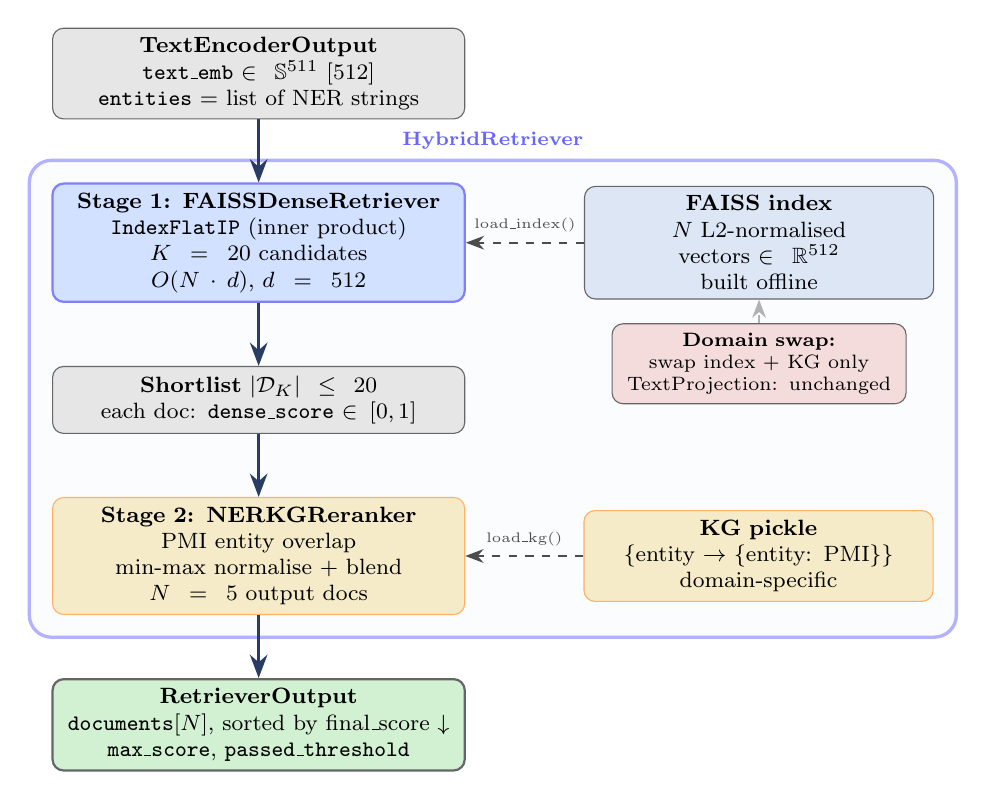
\begin{tikzpicture}[node distance=0.8cm and 1.3cm]

  % Input
  \node[graynode,text width=5cm] (query)
      {\textbf{TextEncoderOutput}\\
       \texttt{text\_emb} $\in \mathbb{S}^{511}$ $[512]$\\
       \texttt{entities} $=$ list of NER strings};

  % Stage 1
  \node[faissnode,text width=5cm,below=of query] (s1)
      {\textbf{Stage 1: FAISSDenseRetriever}\\
       \texttt{IndexFlatIP} (inner product)\\
       $K = 20$ candidates\\
       $O(N \cdot d)$, $d=512$};

  \node[bluenode,text width=4.2cm,right=1.5cm of s1] (faiss_idx)
      {\textbf{FAISS index}\\
       $N$ L2-normalised vectors $\in \mathbb{R}^{512}$\\
       built offline};

  % Shortlist
  \node[graynode,text width=5cm,below=of s1] (shortlist)
      {\textbf{Shortlist} $|\mathcal{D}_K| \leq 20$\\
       each doc: \texttt{dense\_score} $\in [0,1]$};

  % Stage 2
  \node[kgnode,text width=5cm,below=of shortlist] (s2)
      {\textbf{Stage 2: NERKGReranker}\\
       PMI entity overlap\\
       min-max normalise + blend\\
       $N = 5$ output docs};

  \node[kgnode,text width=4.2cm,right=1.5cm of s2] (kg)
      {\textbf{KG pickle}\\
       \{entity $\to$ \{entity: PMI\}\}\\
       domain-specific};

  % Output
  \node[greennode,text width=5cm,below=of s2] (ret_out)
      {\textbf{RetrieverOutput}\\
       \texttt{documents}[$N$], sorted by final\_score $\downarrow$\\
       \texttt{max\_score}, \texttt{passed\_threshold}};

  % Arrows
  \draw[thkarr] (query) -- (s1);
  \draw[thkarr] (s1) -- (shortlist);
  \draw[thkarr] (shortlist) -- (s2);
  \draw[thkarr] (s2) -- (ret_out);
  \draw[arr,dashed] (faiss_idx.west) -- (s1.east)
      node[midway,above,font=\tiny]{load\_index()};
  \draw[arr,dashed] (kg.west) -- (s2.east)
      node[midway,above,font=\tiny]{load\_kg()};

  % Domain swap annotation
  \node[warnnode,font=\scriptsize,text width=3.5cm,
        below=0.3cm of faiss_idx] (swap)
      {\textbf{Domain swap:}\\swap index + KG only\\TextProjection: unchanged};
  \draw[dasharr] (swap.north) -- (faiss_idx.south);

  \begin{pgfonlayer}{background}
    \node[basebox,fill=cBlue!10,draw=blue!30,very thick,rounded corners=8pt,
          fit=(s1)(shortlist)(s2)(faiss_idx)(kg),inner sep=8pt,
          label={[font=\scriptsize\bfseries,text=blue!60]above:HybridRetriever}] {};
  \end{pgfonlayer}

\end{tikzpicture}
\caption{Full two-stage retrieval pipeline. Stage 1 returns $K=20$ candidates
using FAISS; Stage 2 re-scores them with the KG and returns the top $N=5$.
Domain swap replaces only the FAISS index and KG.}
\label{fig:pipeline}
\end{figure}

\subsection{Module Imports}

\begin{lstlisting}[caption={Module imports}]
from abc import ABC, abstractmethod
from dataclasses import dataclass
from typing import List, Optional
import torch
import torch.nn.functional as F
\end{lstlisting}

\begin{table}[H]
\centering
\caption{Import roles}
\begin{tabularx}{\textwidth}{lX}
\toprule
Import & Role \\
\midrule
\texttt{ABC}, \texttt{abstractmethod} & Enforce interface contracts at class definition time \\
\texttt{dataclass} & Auto-generate \texttt{\_\_init\_\_}, \texttt{\_\_repr\_\_} from annotations \\
\texttt{List}, \texttt{Optional} & Static type hints for IDE / mypy checking \\
\texttt{torch}, \texttt{F} & Tensor operations; query embedding originates from a PyTorch model \\
\bottomrule
\end{tabularx}
\end{table}

\begin{remark}[Plain-language]
This module is a two-round library search.
Round~1 (FAISS) is a fast machine that scans every document fingerprint
and picks the 20 closest to your query fingerprint.
Round~2 (KG) is a domain expert who re-reads those 20 shortlisted entries,
checks which ones share key concepts with your query, and promotes the
most relevant 5 to the top.
\end{remark}

%══════════════════════════════════════════════════
\section{Section 1: \texttt{RetrievedDocument} --- Data Transfer Object}
%══════════════════════════════════════════════════

\subsection{Code}

\begin{lstlisting}[caption={\texttt{RetrievedDocument} dataclass}]
@dataclass
class RetrievedDocument:
    doc_id:      str
    text:        str
    image_path:  str
    dense_score: float
    kg_score:    float = 0.0
    final_score: float = 0.0
\end{lstlisting}

\subsection{Field Lifecycle}

\begin{table}[H]
\centering
\caption{\texttt{RetrievedDocument} field population stages}
\begin{tabularx}{\textwidth}{llXl}
\toprule
Field & Type & Populated by & Range \\
\midrule
\texttt{doc\_id}     & \texttt{str}   & Corpus metadata  & --- \\
\texttt{text}        & \texttt{str}   & Corpus metadata  & --- \\
\texttt{image\_path} & \texttt{str}   & Corpus metadata  & \texttt{""} if text-only \\
\texttt{dense\_score}& \texttt{float} & Stage 1 FAISS    & $[0, 1]$ \\
\texttt{kg\_score}   & \texttt{float} & Stage 2 KG       & $[0, 1]$, $0$ if no match \\
\texttt{final\_score}& \texttt{float} & Stage 2 combine  & $[0, 1]$ \\
\bottomrule
\end{tabularx}
\end{table}

\subsection{Final Score Definition}

\begin{definition}[Final Score --- Convex Combination]
The final ranking score for document $i$ is a convex combination of the
normalised dense score and the normalised KG score:
\[
  \boxed{
    \text{final\_score}(i)
    = \alpha \cdot \text{dense\_norm}(i) + (1-\alpha) \cdot \text{kg\_norm}(i),
    \qquad \alpha = 0.7
  }
\]
where both terms are min-max normalised within the Stage 1 shortlist
so they both lie in $[0, 1]$.
\end{definition}

\begin{proposition}[Convexity Guarantees Bounded Score]
Since $\alpha = 0.7 \in (0,1)$, $\text{dense\_norm} \in [0,1]$, and
$\text{kg\_norm} \in [0,1]$:
\[
  \text{final\_score}(i)
  = 0.7 \cdot \text{dense\_norm}(i) + 0.3 \cdot \text{kg\_norm}(i)
  \in [0, 1] \quad \forall\, i
\]
The final score is therefore directly comparable to the domain's
confidence threshold $\tau \in (0,1)$ without any additional scaling.
\end{proposition}

\subsection{Document Lifecycle Diagram}

\begin{figure}[H]
\centering
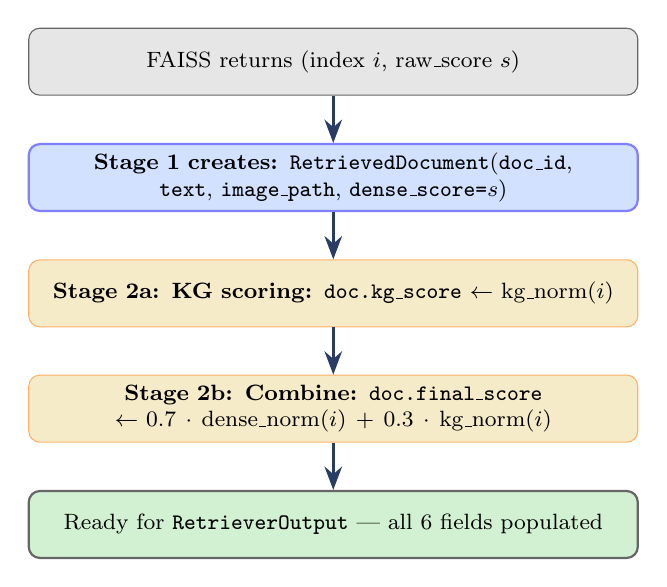
\begin{tikzpicture}[node distance=0.6cm]
  \node[graynode,text width=7.5cm] (s0)
      {FAISS returns (index $i$, raw\_score $s$)};
  \node[faissnode,text width=7.5cm,below=of s0] (s1)
      {\textbf{Stage 1 creates:}
       \texttt{RetrievedDocument}(\texttt{doc\_id}, \texttt{text}, \texttt{image\_path},
       \texttt{dense\_score=}$s$)};
  \node[kgnode,text width=7.5cm,below=of s1] (s2a)
      {\textbf{Stage 2a: KG scoring:}
       \texttt{doc.kg\_score} $\gets$ $\text{kg\_norm}(i)$};
  \node[kgnode,text width=7.5cm,below=of s2a] (s2b)
      {\textbf{Stage 2b: Combine:}
       \texttt{doc.final\_score} $\gets$ $0.7 \cdot \text{dense\_norm}(i) + 0.3 \cdot \text{kg\_norm}(i)$};
  \node[greennode,text width=7.5cm,below=of s2b] (ret)
      {Ready for \texttt{RetrieverOutput} --- all 6 fields populated};

  \foreach \f/\t in {s0/s1,s1/s2a,s2a/s2b,s2b/ret}
    \draw[thkarr] (\f) -- (\t);
\end{tikzpicture}
\caption{Life of a \texttt{RetrievedDocument}: fields are populated
incrementally across the two stages.}
\label{fig:doc_lifecycle}
\end{figure}

\begin{remark}[Plain-language]
This is the \textbf{library card} for one document.
It starts with just the document text and location.
After Stage 1, a ``semantic closeness'' score is added.
After Stage 2, two more scores are added: a concept-overlap score
and a blended final grade.
\end{remark}

%══════════════════════════════════════════════════
\section{Section 2: \texttt{RetrieverOutput} --- Output Envelope}
%══════════════════════════════════════════════════

\subsection{Code}

\begin{lstlisting}[caption={\texttt{RetrieverOutput} dataclass}]
@dataclass
class RetrieverOutput:
    documents:        List[RetrievedDocument]
    query_entities:   List[str]
    max_score:        float
    passed_threshold: bool
\end{lstlisting}

\subsection{Field Specifications}

\begin{table}[H]
\centering
\caption{\texttt{RetrieverOutput} fields and downstream use}
\begin{tabularx}{\textwidth}{llXl}
\toprule
Field & Type & Meaning & Used by \\
\midrule
\texttt{documents}        & \texttt{List[RetrievedDoc]} & Top-$N$ docs sorted by final\_score $\downarrow$ & Generator (LLM context) \\
\texttt{query\_entities}  & \texttt{List[str]}          & NER entities from the query & Diagnostics / logging \\
\texttt{max\_score}       & \texttt{float}              & \texttt{documents[0].final\_score} & Confidence gate \\
\texttt{passed\_threshold}& \texttt{bool}               & $\mathbf{1}[\text{max\_score} \geq \tau]$ & \texttt{pipeline.py} gating \\
\bottomrule
\end{tabularx}
\end{table}

\subsection{Confidence Gate Predicate}

\begin{definition}[Confidence Gate]
\[
  \texttt{passed\_threshold}
  = \mathbf{1}\!\left[\,\max_{i=1}^N \text{final\_score}_i \;\geq\; \tau\,\right],
  \qquad \tau \in (0, 1)
\]
If \texttt{passed\_threshold = False}, \texttt{pipeline.py} rejects or
hedges the answer, preventing hallucinated responses when retrieval quality
is too low.
\end{definition}

\begin{theorem}[Output Contract]
\texttt{RetrieverOutput.documents} is always sorted by \texttt{final\_score}
in descending order, so \texttt{max\_score = documents[0].final\_score}
(or $0.0$ if \texttt{documents} is empty). The generator can safely index
\texttt{documents[0]} as the most relevant document without additional sorting.
\end{theorem}

\begin{remark}[Plain-language]
This is the \textbf{results package} handed to the answer-generator.
It says: ``Here are the best $N$ documents, the search terms we found,
how confident we are in the top result, and whether we are confident
enough to proceed at all.''
\end{remark}

%══════════════════════════════════════════════════
\section{Section 3: Abstract Base Classes}
%══════════════════════════════════════════════════

\subsection{\texttt{BaseDenseRetriever} --- Stage 1 Interface}

\begin{lstlisting}[caption={\texttt{BaseDenseRetriever} ABC}]
class BaseDenseRetriever(ABC):
    @abstractmethod
    def load_index(self, faiss_index_path: str,
                   corpus_metadata_path: str) -> None: pass
    @abstractmethod
    def search(self, query_emb: torch.Tensor,
               top_k: int = 20) -> List[RetrievedDocument]: pass
\end{lstlisting}

\subsection{\texttt{BaseKGReranker} --- Stage 2 Interface}

\begin{lstlisting}[caption={\texttt{BaseKGReranker} ABC}]
class BaseKGReranker(ABC):
    @abstractmethod
    def load_kg(self, kg_path: str) -> None: pass
    @abstractmethod
    def rerank(self, documents: List[RetrievedDocument],
               query_entities: List[str],
               top_n: int = 5) -> List[RetrievedDocument]: pass
\end{lstlisting}

\subsection{ABC Hierarchy Diagram}

\begin{figure}[H]
\centering
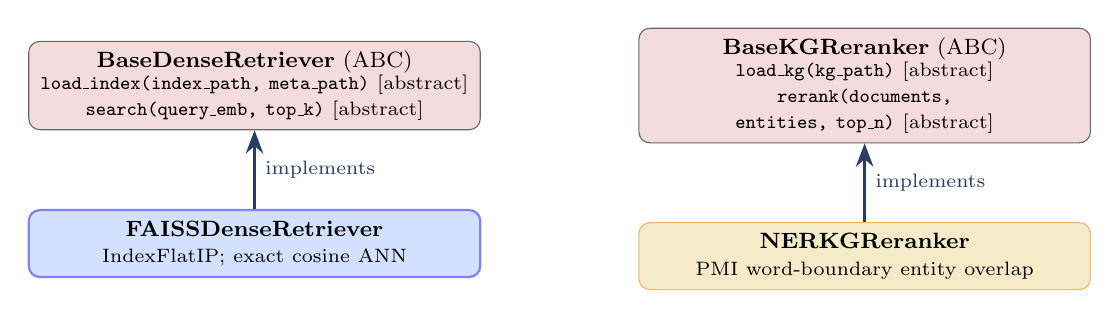
\begin{tikzpicture}[node distance=1.0cm and 2.0cm]
  \node[warnnode,text width=5.5cm] (bdr)
      {\textbf{BaseDenseRetriever} (ABC)\\
       \scriptsize \texttt{load\_index(index\_path, meta\_path)} [abstract]\\
       \texttt{search(query\_emb, top\_k)} [abstract]};

  \node[warnnode,text width=5.5cm,right=2.0cm of bdr] (bkgr)
      {\textbf{BaseKGReranker} (ABC)\\
       \scriptsize \texttt{load\_kg(kg\_path)} [abstract]\\
       \texttt{rerank(documents, entities, top\_n)} [abstract]};

  \node[faissnode,text width=5.5cm,below=1.0cm of bdr] (fdr)
      {\textbf{FAISSDenseRetriever}\\
       \scriptsize IndexFlatIP; exact cosine ANN};

  \node[kgnode,text width=5.5cm,below=1.0cm of bkgr] (nkgr)
      {\textbf{NERKGReranker}\\
       \scriptsize PMI word-boundary entity overlap};

  \draw[thkarr] (fdr.north) -- (bdr.south)
      node[midway,right,font=\scriptsize]{implements};
  \draw[thkarr] (nkgr.north) -- (bkgr.south)
      node[midway,right,font=\scriptsize]{implements};
\end{tikzpicture}
\caption{ABC hierarchy for retriever and re-ranker.}
\label{fig:abc}
\end{figure}

\begin{lemma}[Interface Substitutability]
Any concrete subclass of \texttt{BaseDenseRetriever} (e.g.,
\texttt{FAISSDenseRetriever}, a future \texttt{HNSWRetriever}) can be
swapped into \texttt{HybridRetriever} without changing the orchestrator
--- a direct application of the \emph{Liskov Substitution Principle}.
\end{lemma}

\begin{remark}[Plain-language]
Both ABCs are \textbf{job descriptions}.
\texttt{BaseDenseRetriever} says: ``You must load a search index and
search it.'' \texttt{BaseKGReranker} says: ``You must load a knowledge
graph and re-rank documents.''
Python refuses (\texttt{TypeError}) to hire any class that cannot do
both tasks in its respective role.
\end{remark}

%══════════════════════════════════════════════════
\section{Section 4: \texttt{FAISSDenseRetriever} --- Stage 1}
%══════════════════════════════════════════════════

\subsection{Why \texttt{IndexFlatIP} = Cosine Similarity}

\begin{theorem}[Inner Product = Cosine Similarity for L2-Normalised Vectors]
FAISS \texttt{IndexFlatIP} computes the inner product
$\mathbf{q} \cdot \mathbf{v}_i$ between query $\mathbf{q}$ and every
corpus vector $\mathbf{v}_i$.
When both are L2-normalised ($\|\mathbf{q}\|_2 = \|\mathbf{v}_i\|_2 = 1$):
\[
  \cos(\mathbf{q}, \mathbf{v}_i)
  = \frac{\mathbf{q} \cdot \mathbf{v}_i}{\|\mathbf{q}\|\,\|\mathbf{v}_i\|}
  = \mathbf{q} \cdot \mathbf{v}_i
\]
Therefore \texttt{IndexFlatIP} on L2-normalised vectors is an exact
cosine-similarity search, without any approximation or hash collision.
\end{theorem}

\subsection{\texttt{load\_index} Code and Invariant}

\begin{lstlisting}[caption={\texttt{FAISSDenseRetriever.load\_index()}}]
    def load_index(self, faiss_index_path, corpus_metadata_path):
        import faiss, json
        self.index = faiss.read_index(faiss_index_path)
        with open(corpus_metadata_path, "r") as f:
            self.corpus_metadata = json.load(f)
        assert self.index.ntotal == len(self.corpus_metadata), (
            f"Index size {self.index.ntotal} != "
            f"metadata size {len(self.corpus_metadata)}. "
            "Rebuild index and metadata together."
        )
\end{lstlisting}

\begin{invariant}[Index-Metadata Alignment]
\[
  \forall\, i \in [0, N):\quad
  \text{index.reconstruct}(i) \;\longleftrightarrow\; \text{corpus\_metadata}[i]
\]
Violation (e.g., rebuilding the index without regenerating metadata)
would silently return wrong documents.
The hard \texttt{assert} converts this silent failure into an immediate,
informative error.
\end{invariant}

\subsection{\texttt{search} Code}

\begin{lstlisting}[caption={\texttt{FAISSDenseRetriever.search()}}]
    def search(self, query_emb, top_k=20):
        import numpy as np
        q = query_emb.float().numpy().reshape(1, -1)
        scores, indices = self.index.search(q, top_k)
        scores = scores[0]; indices = indices[0]   # unbatch
        results = []
        for score, idx in zip(scores, indices):
            if idx == -1:
                continue      # FAISS sentinel for empty slot
            meta = self.corpus_metadata[idx]
            results.append(RetrievedDocument(
                doc_id=meta["doc_id"], text=meta["text"],
                image_path=meta.get("image_path", ""),
                dense_score=float(score)))
        return results
\end{lstlisting}

\subsection{Algorithm and Flowchart}

\begin{algorithm}[H]
\caption{\texttt{FAISSDenseRetriever.search}($\mathbf{q}_{\text{emb}}$, $K$)}
\label{alg:faiss_search}
\begin{algorithmic}[1]
\Require $\mathbf{q}_{\text{emb}} \in \mathbb{R}^{512}$, $K \in \mathbb{Z}^+$
\Ensure $\mathcal{D}_K = $ List[\texttt{RetrievedDocument}], sorted by
        \texttt{dense\_score} $\downarrow$, $|\mathcal{D}_K| \leq K$
\State $\mathbf{q} \gets \mathbf{q}_{\text{emb}}.\text{float}().\text{numpy}().\text{reshape}(1, -1)$
       \Comment{Cast to float32, add batch dim $[1, 512]$}
\State $(\mathbf{s},\, \mathbf{idx}) \gets \text{index.search}(\mathbf{q},\, K)$
       \Comment{Exact inner-product; $\mathbf{s}, \mathbf{idx} \in \mathbb{R}^{1 \times K}$}
\State $\mathbf{s} \gets \mathbf{s}[0]$;\; $\mathbf{idx} \gets \mathbf{idx}[0]$
       \Comment{Unbatch: both now $\in \mathbb{R}^K$}
\State $\mathcal{D}_K \gets [\,]$
\ForEach{$(s_j,\, i_j) \in \text{zip}(\mathbf{s},\, \mathbf{idx})$}
  \If{$i_j = -1$} \textbf{continue}
        \Comment{FAISS sentinel: empty slot, skip}
  \EndIf
  \State $\textit{meta} \gets \texttt{corpus\_metadata}[i_j]$
  \State $\mathcal{D}_K.\text{append}\!\left(\texttt{RetrievedDocument}(
         \texttt{doc\_id},\, \texttt{text},\, \texttt{image\_path},\,
         \texttt{dense\_score} = s_j)\right)$
\EndFor
\State \Return $\mathcal{D}_K$
\end{algorithmic}
\end{algorithm}

\begin{figure}[H]
\centering
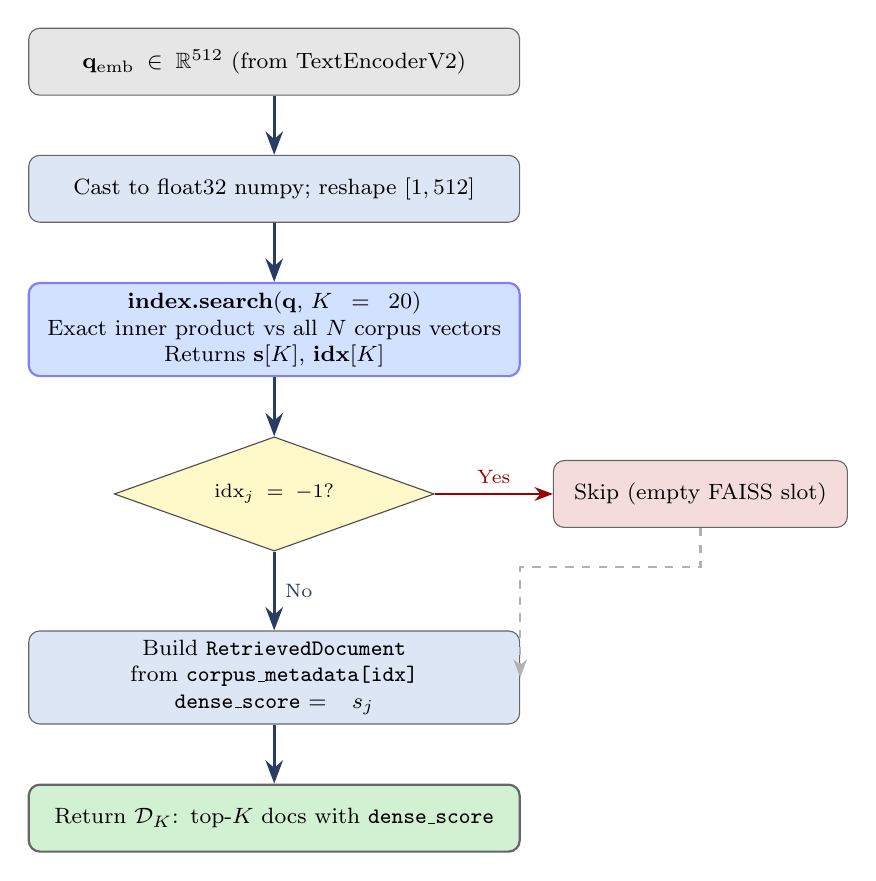
\begin{tikzpicture}[node distance=0.75cm]
  \node[graynode,text width=6cm] (inp)
      {$\mathbf{q}_{\text{emb}} \in \mathbb{R}^{512}$ (from TextEncoderV2)};
  \node[bluenode,text width=6cm,below=of inp] (cast)
      {Cast to float32 numpy; reshape $[1, 512]$};
  \node[faissnode,text width=6cm,below=of cast] (search)
      {\textbf{index.search}($\mathbf{q}$, $K=20$)\\
       Exact inner product vs all $N$ corpus vectors\\
       Returns $\mathbf{s}[K]$, $\mathbf{idx}[K]$};
  \node[decnode,text width=2.5cm,below=of search] (sent)
      {$\text{idx}_j = -1$?};
  \node[warnnode,text width=3.5cm,right=1.5cm of sent] (skip)
      {Skip (empty FAISS slot)};
  \node[bluenode,text width=6cm,below=1.0cm of sent] (build)
      {Build \texttt{RetrievedDocument}\\
       from \texttt{corpus\_metadata[idx]}\\
       \texttt{dense\_score} $= s_j$};
  \node[greennode,text width=6cm,below=of build] (out)
      {Return $\mathcal{D}_K$: top-$K$ docs with \texttt{dense\_score}};

  \draw[thkarr] (inp)--(cast);
  \draw[thkarr] (cast)--(search);
  \draw[thkarr] (search)--(sent);
  \draw[redarr] (sent.east)--(skip.west)
      node[midway,above,font=\scriptsize]{Yes};
  \draw[thkarr] (sent.south)--(build.north)
      node[midway,right,font=\scriptsize]{No};
  \draw[thkarr] (build)--(out);
  \draw[dasharr] (skip.south)--++(0,-0.5)-|(build.east);
\end{tikzpicture}
\caption{\texttt{FAISSDenseRetriever.search()} control flow, including the
FAISS sentinel value guard.}
\label{fig:faiss_search}
\end{figure}

\subsection{Complexity Analysis}

\begin{proposition}[Stage 1 Time Complexity]
\[
  T_{\text{FAISS}} = O(N \cdot d), \quad N = \text{corpus size},\; d = 512
\]
\texttt{IndexFlatIP} is \textbf{exact} (brute-force) --- no approximation
error, but linear in corpus size.
For large corpora ($N > 10^6$), upgrading to \texttt{IndexIVFFlat}
(approximate, faster) would reduce this to $O(\sqrt{N} \cdot d)$.
\end{proposition}

\begin{proposition}[FAISS Sentinel Invariant]
FAISS returns index $= -1$ when fewer than $K$ valid vectors exist in the
index (e.g., when $N < K$).
The \texttt{if idx == -1: continue} guard prevents an out-of-bounds lookup
into \texttt{corpus\_metadata} that would raise an \texttt{IndexError}.
\end{proposition}

\begin{remark}[Plain-language]
Hand the query's 512-number fingerprint to FAISS.
It compares that fingerprint against \emph{every} stored fingerprint in
the corpus and returns the row numbers and scores of the $K$ best matches
--- like a search engine returning the top-$K$ results, but in milliseconds
because it is all matrix multiplication in RAM.
The $-1$ check is a safety valve: ``if FAISS hands back a blank slot, skip it.''
\end{remark}

%══════════════════════════════════════════════════
\section{Section 5: \texttt{NERKGReranker} --- Stage 2}
%══════════════════════════════════════════════════

\subsection{Knowledge Graph Structure}

\begin{definition}[Nested-Dictionary Knowledge Graph]
The KG is a nested dictionary with PMI edge weights:
\[
  \text{KG} = \{
    e_i \to \{ e_j : \text{PMI}(e_i, e_j),\; e_k : \text{PMI}(e_i, e_k),\; \ldots \}
  \}
\]
where nodes $e_i$ are NER entity strings and edge weights are
Pointwise Mutual Information (PMI) scores computed offline from
co-occurrence statistics in the training corpus.
\end{definition}

\begin{definition}[Pointwise Mutual Information]
\[
  \text{PMI}(x, y)
  = \log_2 \frac{P(x, y)}{P(x) \cdot P(y)}
\]
\begin{center}
\begin{tabular}{cc}
\toprule
Value & Interpretation \\
\midrule
$\text{PMI} > 0$ & Co-occur more than chance --- strong semantic link \\
$\text{PMI} = 0$ & Statistically independent \\
$\text{PMI} < 0$ & Anti-correlated (only positive edges stored) \\
\bottomrule
\end{tabular}
\end{center}
\end{definition}

\subsection{Domain Swap: KG Substitution}

\begin{table}[H]
\centering
\caption{Domain-specific KG artefacts}
\begin{tabular}{lllll}
\toprule
Domain & NER model & Corpus & KG entities & \texttt{kg\_path} \\
\midrule
General & spaCy & COCO captions & Common English nouns & \texttt{ner\_kg\_general.pkl} \\
Medical & scispaCy & ROCO / RadLex & Medical terminology & \texttt{ner\_kg\_medical.pkl} \\
\bottomrule
\end{tabular}
\end{table}

\begin{proposition}[Domain-Invariant Re-ranking Algorithm]
Only \texttt{kg\_path} changes between General and Medical domains.
The re-ranking algorithm (\texttt{\_get\_entity\_set}, \texttt{\_score\_document},
\texttt{rerank}) is \textbf{identical} in both domains --- making this a
clean \emph{Strategy} design pattern with swappable data only.
\end{proposition}

\subsection{\texttt{load\_kg} Code}

\begin{lstlisting}[caption={\texttt{NERKGReranker.load\_kg()}}]
    def load_kg(self, kg_path: str) -> None:
        import pickle
        with open(kg_path, "rb") as f:
            self.kg = pickle.load(f)
\end{lstlisting}

\begin{remark}[Plain-language]
The KG is a giant web where each \textbf{node} is a concept
(e.g., ``dog'', ``park'', ``pneumonia'') and each \textbf{edge} has a
number saying how often those two concepts appear together in the training
data. \texttt{load\_kg} loads that web from disk in one line.
\end{remark}

%══════════════════════════════════════════════════
\section{Section 6: \texttt{\_get\_entity\_set()} --- Word-Boundary Matching}
%══════════════════════════════════════════════════

\subsection{Code}

\begin{lstlisting}[caption={\texttt{NERKGReranker.\_get\_entity\_set()}}]
    def _get_entity_set(self, text: str) -> set:
        import re
        if self.kg is None:
            return set()
        found = set()
        lower_text = text.lower()
        for entity in self.kg:
            pattern = r'\b' + re.escape(entity.lower()) + r'\b'
            if re.search(pattern, lower_text):
                found.add(entity)
        return found
\end{lstlisting}

\subsection{Mathematical Definition and Theorem}

\begin{definition}[Word-Boundary Match Indicator]
For entity $e$ and document text $t$:
\[
  \text{match}(e, t)
  = \begin{cases}
    1 & \text{if regex } \texttt{\textbackslash b} + e + \texttt{\textbackslash b}
        \text{ appears in } t_{\text{lower}} \\
    0 & \text{otherwise}
  \end{cases}
\]
The $\texttt{\textbackslash b}$ \emph{word-boundary assertion} ensures we match
whole tokens only, not substrings.
\end{definition}

\begin{theorem}[Substring False Positive Prevention]
Without word-boundary anchors, entity ``cat'' would match inside
``category'' and ``scatter''; entity ``dog'' would match inside ``dogmatic''.
With $\texttt{\textbackslash b}$ anchors, only standalone occurrences match:
\[
  \text{match}(\texttt{"cat"}, \texttt{"a cat sat"}) = 1 \quad \checkmark
\]
\[
  \text{match}(\texttt{"cat"}, \texttt{"scattered category"}) = 0
  \quad \checkmark \text{ (prevented false positive)}
\]
This prevents inflated KG scores from accidental substring matches,
which would corrupt the Stage 2 ranking.
\end{theorem}

\begin{figure}[H]
\centering
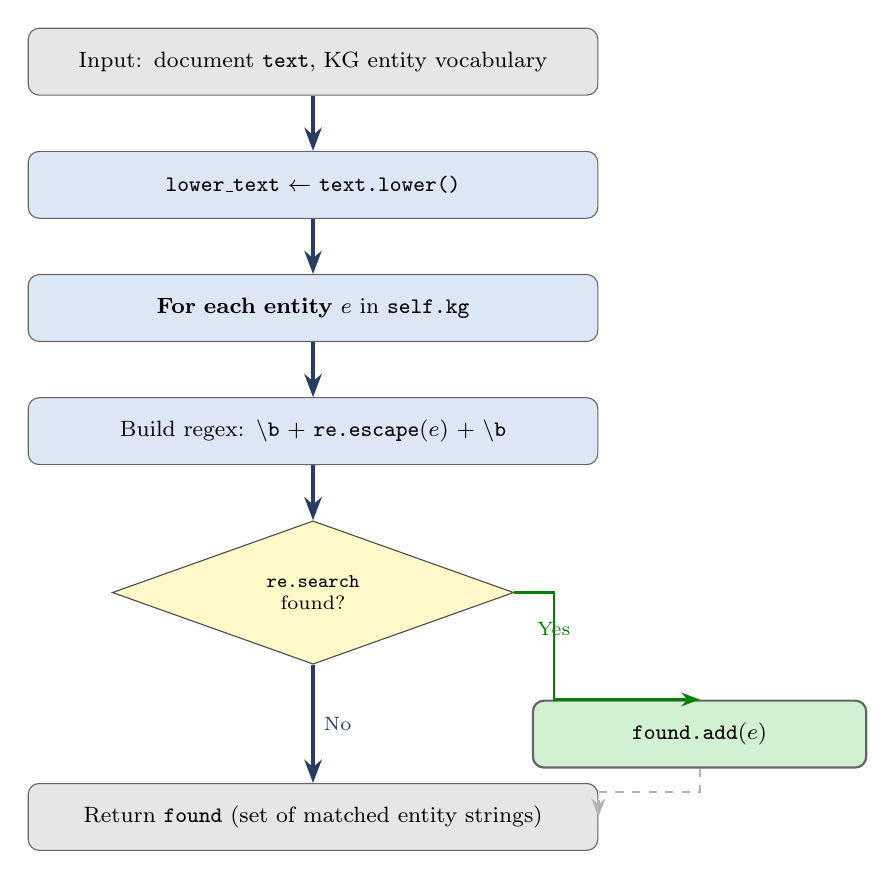
\begin{tikzpicture}[node distance=0.7cm]
  \node[graynode,text width=7cm] (inp)
      {Input: document \texttt{text}, KG entity vocabulary};
  \node[bluenode,text width=7cm,below=of inp] (lower)
      {\texttt{lower\_text} $\gets$ \texttt{text.lower()}};
  \node[bluenode,text width=7cm,below=of lower] (loop)
      {\textbf{For each entity} $e$ in \texttt{self.kg}};
  \node[bluenode,text width=7cm,below=of loop] (pat)
      {Build regex: \texttt{\textbackslash b} + \texttt{re.escape}($e$) + \texttt{\textbackslash b}};
  \node[decnode,text width=3cm,below=of pat] (match)
      {\texttt{re.search}\\found?};
  \node[greennode,text width=4cm,below right=0.9cm and 1.5cm of match] (add)
      {\texttt{found.add}($e$)};
  \node[graynode,text width=7cm,below=1.5cm of match] (ret)
      {Return \texttt{found} (set of matched entity strings)};

  \draw[thkarr] (inp)--(lower);
  \draw[thkarr] (lower)--(loop);
  \draw[thkarr] (loop)--(pat);
  \draw[thkarr] (pat)--(match);
  \draw[grnarr] (match.east)--++(0.5,0)|-(add.north)
      node[near start,above,font=\scriptsize]{Yes};
  \draw[dasharr] (add.south)--++(0,-0.3)-|(ret.east);
  \draw[thkarr] (match.south)--(ret.north)
      node[midway,right,font=\scriptsize]{No};
\end{tikzpicture}
\caption{\texttt{\_get\_entity\_set()} control flow. For each KG entity,
a word-boundary regex is tested against the lowercased document text.}
\label{fig:entity_set}
\end{figure}

\begin{remark}[Plain-language]
We scan the document text looking for each concept word from the KG ---
but we insist it must appear as a \textbf{standalone word}, not buried
inside another word.
Without this guard, searching for ``cat'' would wrongly trigger on
``category'' or ``scatter'' --- corrupting the KG score.
\texttt{re.escape} also handles entities containing special characters
(e.g., ``x-ray'' containing a hyphen) without crashing the regex engine.
\end{remark}

%══════════════════════════════════════════════════
\section{Section 7: \texttt{\_score\_document()} --- PMI-Weighted Entity Overlap}
%══════════════════════════════════════════════════

\subsection{Code}

\begin{lstlisting}[caption={\texttt{NERKGReranker.\_score\_document()}}]
    def _score_document(self, doc_text: str, query_entities: set) -> float:
        if not query_entities or self.kg is None:
            return 0.0
        doc_entities = self._get_entity_set(doc_text)
        score = 0.0
        for q_ent in query_entities:
            if q_ent not in self.kg:
                continue
            for d_ent in doc_entities:
                if d_ent in self.kg[q_ent]:
                    score += self.kg[q_ent][d_ent]   # PMI weight
        return score
\end{lstlisting}

\subsection{Mathematical Formulation}

\begin{lemma}[Bipartite PMI-Weighted Entity Overlap Score]
Let $Q$ be the set of NER entities from the query and
$D(\text{doc})$ be the set of KG entities matched in a document.
The raw KG score is:
\[
  \text{score\_raw}(\text{doc})
  = \sum_{q \in Q} \sum_{d \in D(\text{doc})}
    \text{PMI}(q, d)
    \cdot \mathbf{1}\!\left[d \in \text{KG}[q]\right]
\]
Properties:
\begin{enumerate}
  \item Score $= 0$ if $Q = \emptyset$ or KG is not loaded $\to$ falls back to dense-only ranking.
  \item Score $= 0$ if no KG edge connects any query entity to any document entity.
  \item Score is \emph{unnormalised} at this stage; normalisation happens in \texttt{rerank()}.
  \item Complexity: $O(|Q| \cdot |D(\text{doc})|)$ --- bounded by shortlist entities, not full KG size.
\end{enumerate}
\end{lemma}

\subsection{PMI Score Interaction Diagram}

\begin{figure}[H]
\centering
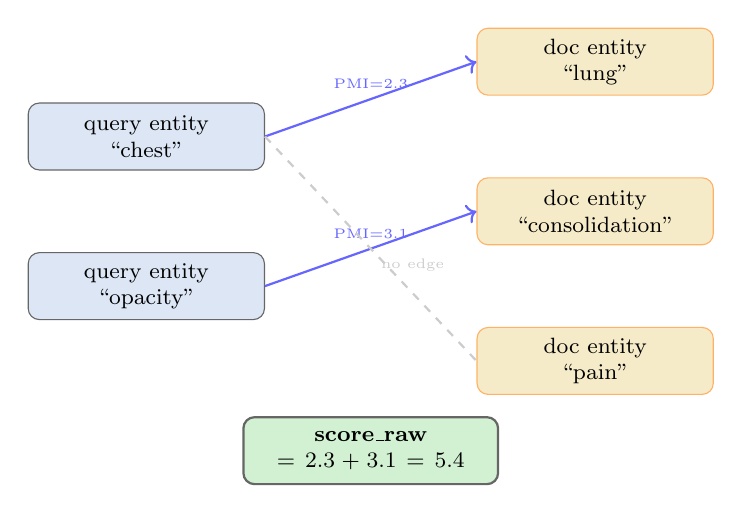
\begin{tikzpicture}[scale=0.95]

  % Query entities
  \node[bluenode,text width=2.5cm] (q1) at (0, 2) {query entity\\``chest''};
  \node[bluenode,text width=2.5cm] (q2) at (0, 0) {query entity\\``opacity''};

  % Doc entities
  \node[kgnode,text width=2.5cm] (d1) at (6, 3) {doc entity\\``lung''};
  \node[kgnode,text width=2.5cm] (d2) at (6, 1) {doc entity\\``consolidation''};
  \node[kgnode,text width=2.5cm] (d3) at (6,-1) {doc entity\\``pain''};

  % PMI edges
  \draw[thick,blue!60,->] (q1.east) -- node[above,font=\tiny]{PMI=2.3} (d1.west);
  \draw[thick,blue!60,->] (q2.east) -- node[above,font=\tiny]{PMI=3.1} (d2.west);
  \draw[thick,gray!40,dashed] (q1.east) -- node[below right,font=\tiny]{no edge} (d3.west);

  % Score
  \node[greennode,text width=3cm] at (3, -2.2) {
      \textbf{score\_raw} $= 2.3 + 3.1 = 5.4$};

\end{tikzpicture}
\caption{PMI bipartite matching between query entities (left) and document
entities (right). Only edges present in the KG contribute to the raw score.}
\label{fig:pmi_bipartite}
\end{figure}

\begin{remark}[Plain-language]
For every concept in the query and every concept in the document, look up
their ``togetherness score'' (PMI) in the KG and add them all up.
A document mentioning many concepts known to co-occur with the query's
concepts gets a high raw score --- even if the exact query words are absent.
\end{remark}

%══════════════════════════════════════════════════
\section{Section 8: \texttt{rerank()} --- Full Re-ranking Algorithm}
%══════════════════════════════════════════════════

\subsection{Code}

\begin{lstlisting}[caption={\texttt{NERKGReranker.rerank()}}]
    def rerank(self, documents, query_entities, top_n=5):
        if not documents: return []
        query_entity_set = set(query_entities)
        # 1. Min-max normalise dense scores within shortlist
        dense_scores = [d.dense_score for d in documents]
        min_s, max_s = min(dense_scores), max(dense_scores)
        score_range = max_s - min_s if max_s > min_s else 1.0
        # 2. Compute KG scores
        kg_scores = [self._score_document(d.text, query_entity_set)
                     for d in documents]
        # 3. Normalise KG scores to [0,1]
        max_kg = max(kg_scores) if max(kg_scores) > 0 else 1.0
        kg_scores_norm = [s / max_kg for s in kg_scores]
        # 4. Combine and sort
        for doc, kg_n, dense_s in zip(documents, kg_scores_norm, dense_scores):
            dense_n = (dense_s - min_s) / score_range
            doc.kg_score    = kg_n
            doc.final_score = 0.7 * dense_n + 0.3 * kg_n
        documents.sort(key=lambda d: d.final_score, reverse=True)
        return documents[:top_n]
\end{lstlisting}

\subsection{Mathematical Formulation}

\begin{definition}[Min-Max Normalisation]
\[
  \text{dense\_norm}(i) =
  \frac{\text{dense}_i - \min_j \text{dense}_j}
       {\max_j \text{dense}_j - \min_j \text{dense}_j}
  \in [0, 1]
\]
\[
  \text{kg\_norm}(i) =
  \frac{\text{score\_raw}(i)}{\max_j \text{score\_raw}(j)}
  \in [0, 1]
\]
\end{definition}

\begin{definition}[Combined Final Score]
\[
  \text{final\_score}(i) =
  \underbrace{0.7}_{\alpha} \cdot \text{dense\_norm}(i) +
  \underbrace{0.3}_{1-\alpha} \cdot \text{kg\_norm}(i)
\]
with $\alpha = \texttt{DENSE\_WEIGHT} = 0.7$.
\end{definition}

\subsection{Full Algorithm}

\begin{algorithm}[H]
\caption{\texttt{NERKGReranker.rerank}($\mathcal{D}_K$, $Q$, $N$)}
\label{alg:rerank}
\begin{algorithmic}[1]
\Require Shortlist $\mathcal{D}_K$ (Stage~1 output), query entities $Q$,
         $N$ = desired output count
\Ensure Top-$N$ \texttt{RetrievedDocument}s sorted by \texttt{final\_score} $\downarrow$
\If{$\mathcal{D}_K = \emptyset$} \Return $[\,]$ \EndIf

\State \textbf{--- Step 1: Min-max normalise dense scores ---}
\State $s_{\min} \gets \min_i \text{dense}_i$;\;
       $s_{\max} \gets \max_i \text{dense}_i$
\State $\text{range} \gets (s_{\max} - s_{\min})$ if $s_{\max} \neq s_{\min}$ else $1.0$
       \Comment{Guard: all-equal $\to$ range = 1.0}

\State \textbf{--- Step 2: Compute raw KG scores ---}
\ForEach{$d \in \mathcal{D}_K$}
  \State $r_d \gets \textsc{\_score\_document}(d.\texttt{text},\, Q)$
\EndFor

\State \textbf{--- Step 3: Normalise KG scores ---}
\State $r_{\max} \gets \max_d r_d$ if $\max_d r_d > 0$ else $1.0$
       \Comment{Guard: no KG match $\to$ all-zero}
\State $\text{kg\_norm}_d \gets r_d / r_{\max}$ for each $d$

\State \textbf{--- Step 4: Combine and sort ---}
\ForEach{$d \in \mathcal{D}_K$}
  \State $\text{dense\_norm}_d \gets (d.\texttt{dense\_score} - s_{\min}) / \text{range}$
  \State $d.\texttt{kg\_score} \gets \text{kg\_norm}_d$
  \State $d.\texttt{final\_score}
         \gets 0.7 \cdot \text{dense\_norm}_d + 0.3 \cdot \text{kg\_norm}_d$
\EndFor
\State Sort $\mathcal{D}_K$ by $\texttt{final\_score}$ descending
\State \Return $\mathcal{D}_K[:N]$
\end{algorithmic}
\end{algorithm}

\subsection{Edge-Case Handling}

\begin{table}[H]
\centering
\caption{Edge cases and guards in \texttt{rerank()}}
\begin{tabularx}{\textwidth}{lXX}
\toprule
Condition & Guard & Effect \\
\midrule
All dense scores equal & \texttt{range = 1.0} & \texttt{dense\_norm = 0} for all $\to$ KG drives ranking \\
No KG entity matches & \texttt{max\_kg = 1.0} & \texttt{kg\_norm = 0} for all $\to$ dense drives ranking \\
Empty shortlist & \texttt{return []} & No division-by-zero \\
$N >$ shortlist size & \texttt{documents[:N]} & Returns fewer than $N$ (Python slice is safe) \\
\bottomrule
\end{tabularx}
\end{table}

\subsection{rerank Scoring Flowchart}

\begin{figure}[H]
\centering
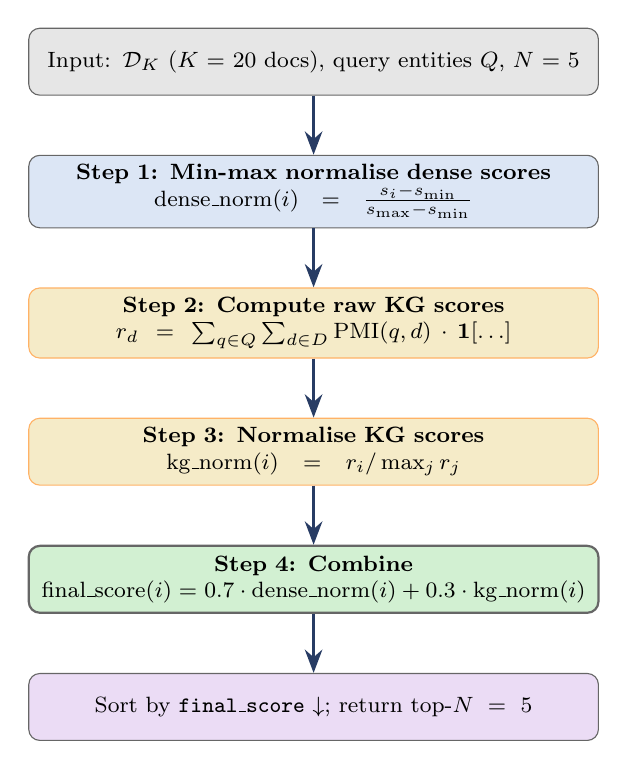
\begin{tikzpicture}[node distance=0.75cm]

  \node[graynode,text width=7cm] (inp)
      {Input: $\mathcal{D}_K$ ($K=20$ docs), query entities $Q$, $N=5$};

  \node[bluenode,text width=7cm,below=of inp] (minmax)
      {\textbf{Step 1: Min-max normalise dense scores}\\
       $\text{dense\_norm}(i) = \frac{s_i - s_{\min}}{s_{\max} - s_{\min}}$};

  \node[kgnode,text width=7cm,below=of minmax] (kgraw)
      {\textbf{Step 2: Compute raw KG scores}\\
       $r_d = \sum_{q \in Q} \sum_{d \in D} \text{PMI}(q,d) \cdot \mathbf{1}[\ldots]$};

  \node[kgnode,text width=7cm,below=of kgraw] (kgnorm)
      {\textbf{Step 3: Normalise KG scores}\\
       $\text{kg\_norm}(i) = r_i / \max_j r_j$};

  \node[greennode,text width=7cm,below=of kgnorm] (combine)
      {\textbf{Step 4: Combine}\\
       $\text{final\_score}(i) = 0.7 \cdot \text{dense\_norm}(i)
       + 0.3 \cdot \text{kg\_norm}(i)$};

  \node[purplenode,text width=7cm,below=of combine] (sort)
      {Sort by \texttt{final\_score} $\downarrow$; return top-$N=5$};

  \foreach \f/\t in {inp/minmax,minmax/kgraw,kgraw/kgnorm,kgnorm/combine,combine/sort}
    \draw[thkarr] (\f) -- (\t);

\end{tikzpicture}
\caption{\texttt{rerank()} 4-step scoring pipeline. Normalisation ensures both
judges (dense, KG) operate on the same $[0,1]$ scale before blending.}
\label{fig:rerank_flow}
\end{figure}

\begin{lemma}[Normalisation Ensures Score Comparability]
Without min-max normalisation, the dense scores (cosine similarities $\in [0,1]$)
and KG scores (sum of PMI values $\in [0, \infty)$) are on incompatible scales.
Normalising both to $[0,1]$ before the convex combination ensures the
$\alpha = 0.7$ / $1{-}\alpha = 0.3$ weights reflect the intended importance,
not the arbitrary magnitude of the raw scores.
\end{lemma}

\begin{remark}[Plain-language: Two Judges]
Think of \textbf{two judges} scoring contestants:
\textbf{Judge 1} (FAISS) gives raw semantic similarity scores ---
but they vary widely, so we rescale the best to 1.0 and worst to 0.0 first.
\textbf{Judge 2} (KG) gives concept-overlap scores --- also rescaled to $[0,1]$.
\textbf{Final verdict}: Judge 1 counts 70\%, Judge 2 counts 30\%.
Sort by final verdict, keep the top $N$.
\end{remark}

%══════════════════════════════════════════════════
\section{Section 9: \texttt{HybridRetriever} --- Façade Orchestrator}
%══════════════════════════════════════════════════

\subsection{Code}

\begin{lstlisting}[caption={\texttt{HybridRetriever} class}]
class HybridRetriever:
    def __init__(self):
        self.dense    = FAISSDenseRetriever()
        self.reranker = NERKGReranker()

    def load(self, domain_config) -> None:
        self.dense.load_index(domain_config.faiss_index_path,
                              domain_config.corpus_metadata_path)
        self.reranker.load_kg(domain_config.kg_path)

    def retrieve(self, text_encoder_output, domain_config) -> RetrieverOutput:
        shortlist = self.dense.search(
            query_emb=text_encoder_output.text_emb,
            top_k=domain_config.dense_top_k)
        top_n_docs = self.reranker.rerank(
            documents=shortlist,
            query_entities=text_encoder_output.entities,
            top_n=domain_config.rerank_top_n)
        max_score = top_n_docs[0].final_score if top_n_docs else 0.0
        passed    = max_score >= domain_config.confidence_threshold
        return RetrieverOutput(documents=top_n_docs,
                               query_entities=text_encoder_output.entities,
                               max_score=max_score,
                               passed_threshold=passed)
\end{lstlisting}

\subsection{Façade Pattern}

\begin{definition}[Façade Design Pattern]
\texttt{HybridRetriever} is a \emph{Façade}: it exposes a single, simple
\texttt{retrieve()} API that hides the two-stage complexity.
\texttt{pipeline.py} calls only \texttt{retriever.retrieve()} and
\texttt{retriever.load()} --- it never directly interacts with
\texttt{FAISSDenseRetriever} or \texttt{NERKGReranker}.
\end{definition}

\subsection{Full Orchestration Algorithm}

\begin{algorithm}[H]
\caption{\texttt{HybridRetriever.retrieve}(\textit{text\_out}, $\delta$)}
\label{alg:hybrid_retrieve}
\begin{algorithmic}[1]
\Require \texttt{text\_out.text\_emb} $\in \mathbb{S}^{511}$,
         \texttt{text\_out.entities} $= Q$,
         domain config $\delta$ with $K$, $N$, $\tau$
\Ensure \texttt{RetrieverOutput}

\State \textbf{--- Stage 1: Dense FAISS search ---}
\State $\mathcal{D}_K \gets \text{dense.search}(\mathbf{e}_t,\; K = \delta.\texttt{dense\_top\_k})$
       \Comment{$|\mathcal{D}_K| \leq K$; dense\_score populated}

\State \textbf{--- Stage 2: KG re-rank ---}
\State $\mathcal{D}_N \gets \text{reranker.rerank}(\mathcal{D}_K,\; Q,\; N = \delta.\texttt{rerank\_top\_n})$
       \Comment{$|\mathcal{D}_N| \leq N$; kg\_score + final\_score populated}

\State \textbf{--- Confidence gate ---}
\State $s_{\max} \gets \mathcal{D}_N[0].\texttt{final\_score}$
       if $\mathcal{D}_N \neq \emptyset$ else $0.0$
\State $\text{passed} \gets (s_{\max} \geq \tau)$
       \Comment{$\tau = \delta.\texttt{confidence\_threshold}$}

\State \Return $\texttt{RetrieverOutput}(\mathcal{D}_N,\; Q,\; s_{\max},\; \text{passed})$
\end{algorithmic}
\end{algorithm}

\subsection{Full HybridRetriever Flowchart}

\begin{figure}[H]
\centering
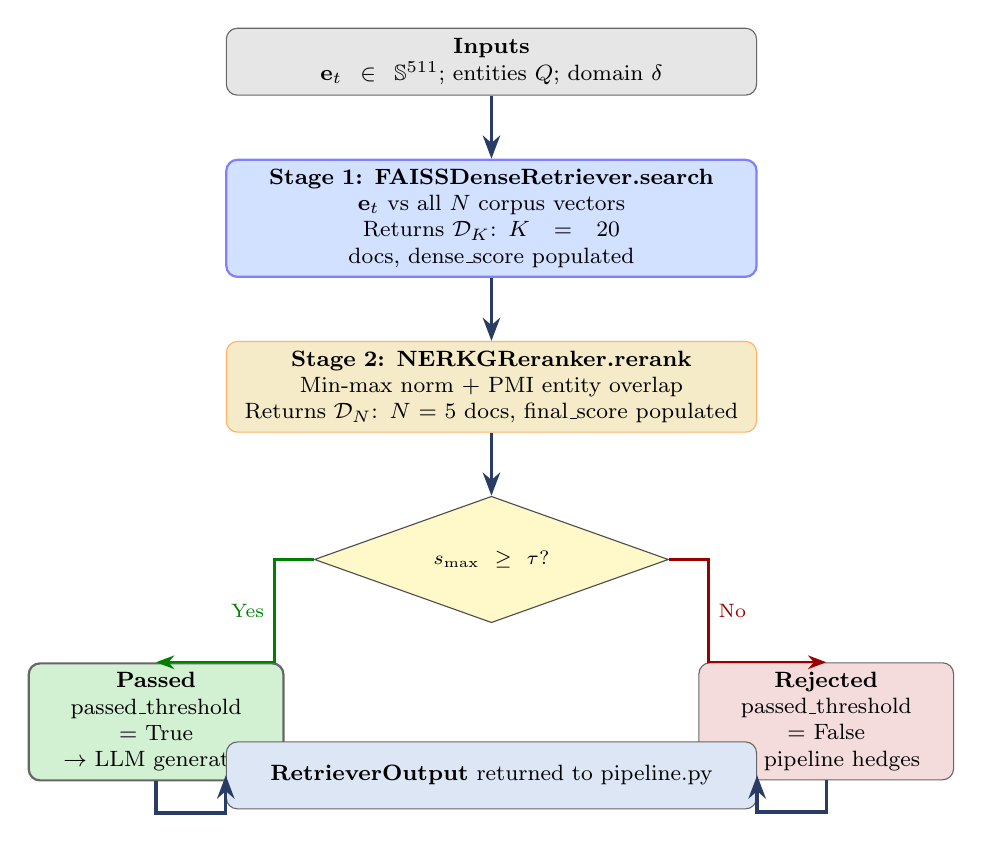
\begin{tikzpicture}[node distance=0.8cm]

  \node[graynode,text width=6.5cm] (inp)
      {\textbf{Inputs}\\
       $\mathbf{e}_t \in \mathbb{S}^{511}$; entities $Q$; domain $\delta$};

  \node[faissnode,text width=6.5cm,below=of inp] (stage1)
      {\textbf{Stage 1: FAISSDenseRetriever.search}\\
       $\mathbf{e}_t$ vs all $N$ corpus vectors\\
       Returns $\mathcal{D}_K$: $K=20$ docs, dense\_score populated};

  \node[kgnode,text width=6.5cm,below=of stage1] (stage2)
      {\textbf{Stage 2: NERKGReranker.rerank}\\
       Min-max norm + PMI entity overlap\\
       Returns $\mathcal{D}_N$: $N=5$ docs, final\_score populated};

  \node[decnode,text width=3cm,below=of stage2] (gate)
      {$s_{\max} \geq \tau$?};

  \node[greennode,text width=3cm,below left=0.9cm and 1.5cm of gate] (pass)
      {\textbf{Passed}\\passed\_threshold = True\\$\to$ LLM generates};
  \node[warnnode,text width=3cm,below right=0.9cm and 1.5cm of gate] (fail)
      {\textbf{Rejected}\\passed\_threshold = False\\$\to$ pipeline hedges};

  \node[bluenode,text width=6.5cm,below=1.5cm of gate] (out)
      {\textbf{RetrieverOutput} returned to pipeline.py};

  \draw[thkarr] (inp)--(stage1);
  \draw[thkarr] (stage1)--(stage2);
  \draw[thkarr] (stage2)--(gate);
  \draw[grnarr] (gate.west)--++(-0.5,0)|-(pass.north)
      node[near start,left,font=\scriptsize]{Yes};
  \draw[redarr] (gate.east)--++(0.5,0)|-(fail.north)
      node[near start,right,font=\scriptsize]{No};
  \draw[thkarr] (pass.south)--++(0,-0.4)-|(out.west);
  \draw[thkarr] (fail.south)--++(0,-0.4)-|(out.east);

\end{tikzpicture}
\caption{\texttt{HybridRetriever.retrieve()} end-to-end flow.
Both Stage 1 and Stage 2 feed into a confidence gate before the output
is returned to \texttt{pipeline.py}.}
\label{fig:hybrid_flow}
\end{figure}

\begin{remark}[Plain-language]
The \textbf{manager} coordinates both stages:
\begin{enumerate}
  \item Tells Stage 1: ``find me the 20 closest documents.''
  \item Hands those 20 to Stage 2: ``re-rank by concept overlap, keep the best 5.''
  \item Checks: ``is the top score high enough to trust?''
  \item Packages everything up and returns it to the answer generator.
\end{enumerate}
\end{remark}

%══════════════════════════════════════════════════
\section{Summary: Hyperparameters, Complexity, and Domain Swap}
%══════════════════════════════════════════════════

\subsection{Hyperparameter Reference}

\begin{table}[H]
\centering
\caption{Complete hyperparameter reference}
\begin{tabularx}{\textwidth}{llXl}
\toprule
Symbol & Config key & Meaning & Default \\
\midrule
$d$ & --- & Embedding dimensionality & 512 \\
$K$ & \texttt{dense\_top\_k} & FAISS shortlist size & 20 \\
$N$ & \texttt{rerank\_top\_n} & Final output size & 5 \\
$\alpha$ & \texttt{DENSE\_WEIGHT} & Dense score weight & 0.7 \\
$1{-}\alpha$ & \texttt{KG\_WEIGHT} & KG score weight & 0.3 \\
$\tau$ & \texttt{confidence\_threshold} & Pass/fail threshold & domain-specific \\
\bottomrule
\end{tabularx}
\end{table}

\subsection{Time Complexity per Query}

\begin{table}[H]
\centering
\caption{Time complexity analysis}
\begin{tabularx}{\textwidth}{lXl}
\toprule
Stage & Complexity & Notes \\
\midrule
Stage 1 --- FAISS search & $O(N \cdot d)$ & Exact brute-force; $N$ = corpus size \\
Stage 2 --- Entity matching & $O(K \cdot |\text{KG}|)$ & Regex over $K$ docs \\
Stage 2 --- Scoring \& sort & $O(K \cdot |Q| \cdot |D|) + O(K \log K)$ & $|Q|$, $|D|$: entity set sizes \\
\textbf{Overall} & $O(N \cdot d)$ & Dominated by FAISS for large $N$ \\
\bottomrule
\end{tabularx}
\end{table}

\subsection{Domain Swap Summary}

\begin{table}[H]
\centering
\caption{Domain swap: what changes and what does not}
\begin{tabularx}{\textwidth}{lXX}
\toprule
Artefact & General Domain & Medical Domain \\
\midrule
FAISS index & COCO 512-d embeddings & ROCO 512-d embeddings \\
KG pickle & spaCy NER + COCO PMI & scispaCy + RadLex PMI \\
NER entity vocab & General English nouns & Medical terminology (21 terms) \\
\texttt{TextProjection} weights & \textbf{Shared (unchanged)} & \textbf{Shared (unchanged)} \\
Re-ranking algorithm & \textbf{Identical} & \textbf{Identical} \\
\bottomrule
\end{tabularx}
\end{table}

\begin{corollary}[Retrieval Algorithm Domain-Invariance]
The retrieval algorithms (\texttt{FAISSDenseRetriever.search},
\texttt{NERKGReranker.rerank}) are completely domain-independent.
Only the data artefacts (FAISS index, KG pickle) change on domain swap.
This confirms the core thesis claim: the shared 512-d embedding space
enables domain-agnostic retrieval with only corpus-level substitution.
\end{corollary}

\end{document}
